%sources
\chapter{Event Topology and Datasets}

%what are the best sources and why\\
%probability of being of astrophysical origin\\
%History of EHE, HESE to bronze, gold alerts Thomas Kintschers gfu\\
%what is a gfu\\
%hängt ab von zen, dec, track\_len, bdt\_up (upgoing oder nicht) oder bei donwgoing: truncated energy, qtot (deponierte Ladung)\\
%\_zen\_cut = np.radians(82.)\\
%up: pass\_gold[m]   = pass\_precut[m] \& (qtot[m] > 10.\*\*np.polyval(\_coeff2, np.sin(dec[m])))\\
%\_coeff2 = [  -4.06580, -10.60906,  -9.61048,   3.01219 ]\\
%down: pass\_gold[m]   \= pass\_precut[m] \& (logTruncated[m] > \_cut2)\\
%\_cut2   = 5.14\\
%
%table of sources, skymaps\\

Historically events were categorized between high energy starting events (HESE) and extremely high energy events (EHE).
Starting events are as the name suggests events starting inside the detector volume (interaction vertex)

Besides a few tweaks to the HESE and EHE channels, the new alert system introduced a breakdown into two different categories of events based on their probability of being of atrophysical origin.
These are called gold and bronze events, with gold having at least a $\SI{50}{\percent}$ astrophysical purity in comparison to $\SI{30}{\percent}$ for bronze events.
The latter were introduced to satisfy the demand for even more alerts.
This new system also features a new event type, the Gamma-Ray-Followup (GFU), which is highest in the event categorization hierarchy, meaning that if an event is classified as a GFU event it is also possible for the event to be a HESE or EHE event additionally.
This hierarchy is based on studies for angular resolution and astrophysical purity making GFU gold events the first stop for a search for astrophysical neutrino sources.

\cite{Aartsen_2017}

\section{Gamma-Ray-Followup}

The Gamma-Ray-Followup track selection, GFU for short, is a pretrained binary decision tree (BDT) identifying through going single track events from all directions that are likely neutrino induced.
The required astrophysical purity of at least $\SI{50}{\percent}$ for the gold selection is obtained by tight cuts on muon energy and deposited charge.\\
The BDT consists of two basic cuts different for each hemisphere.
Both, for upgoing and downgoing events, use a precut which is more like a sanity check outruling invalid events.
All events having a tracklength greater than $\SI{0}{\meter}$ and a truncated energy greater than $\SI{0}{\electronvolt}$ pass this selection.
Additionally all events have to be between $\SI{82}{\radian}$ and $\SI{-82}{\radian}$ zenith.
Events from the northern sky must have a truncated energy higher than $\SI{1e5.14}{\giga\electronvolt}$ to pass the GFU selection.
In the southern hemisphere, the deposited charge ($qtot$) of the events must meet the following condition as a function $d$,
\begin{equation}
  \log_{10}(qtot) > -4.06580\cdot d^3 - 10.60906\cdot d^2  -9.61048\cdot d + 3.01219,
\end{equation}
where $d$ is the sine of the declination of the events.
The individual signalness is obtained through a grid interpolation based on the position of these events.

\subsection{Sources}

The selected sources in this analysis are part of the alert catalogue version 2 which features about 300 alerts in total.
The GFU-gold alerts used as sources are displayed in table \ref{tab:sources}.
These events are also visible in figure \ref{fig:skymap_1}.
All events used are in an energy range of $\SI{174}{\tera\electronvolt}$ to $\SI{5960}{\tera\electronvolt}$.
The sources used in the later introduced time-dependent analysis are shown in figure \ref{fig:skymap_2}.
It is worth mentioning that the time integrated analysis uses all sources listed in the table \ref{tab:sources}, regardless of the time interval of the dataset used.
The sources in the time-dependent analysis, on the other hand, are all temporally located in the dataset presented in the chapter \ref{sec:data} and can additionally be seen in table \ref{tab:sources_time_dep}.

\begin{figure}
    \centering
    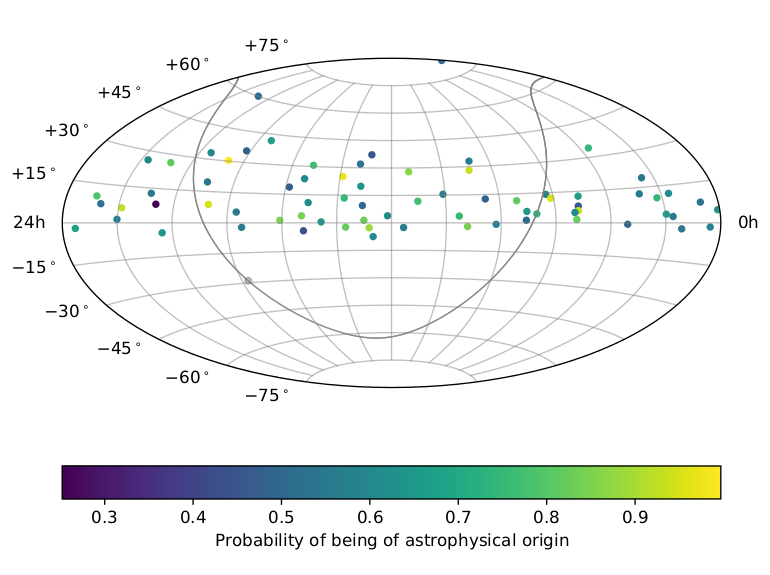
\includegraphics[draft=true,width=\linewidth]{Plots/02_sources/gfu_gold_skymap.pdf}
    \label{fig:skymap_1}
    \caption{skymap time int.}
\end{figure}

\begin{figure}
    \centering
    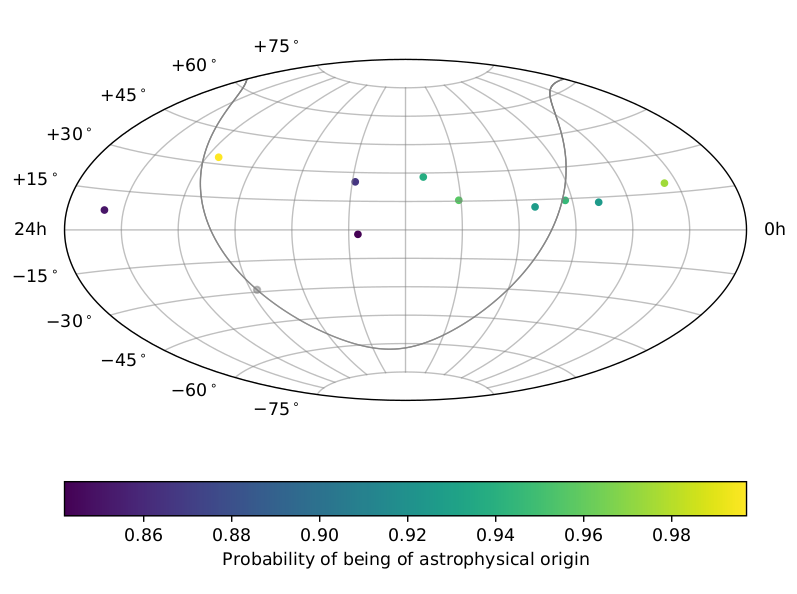
\includegraphics[draft=true,width=\linewidth]{Plots/02_sources/gfu_gold_skymap_time_dep.pdf}
    \label{fig:skymap_2}
    \caption{skymap time dep.}
\end{figure}

\begin{table}[!htb]
  \caption{Table of the 72 GFU-gold events used as sources in this analysis. Shown are the features time in MJD, declination $\delta$ in degrees and right ascension $\alpha$ also in degrees. The time-dependent analysis uses a subset of these sources. The order of the sources corresponds to the processing order in the analysis pipeline.}
  \label{tab:sources}
  \begin{subtable}{.5\linewidth}
  \centering
  \begin{tabular}{ccrr}
    \toprule
    Nr. & MJD &  $\delta$ in $\si{\degree}$ & $\alpha$ in $\si{\degree}$ \\
    \toprule
    1 & 55695.06 & -0.03 & 2.42 \\ 2 & 57709.33 & 0.03 & 1.37 \\ 3 & 57284.21 & 0.53 & 4.88 \\ 4 & 58806.04 & 0.07 & 4.0 \\ 5 & 56927.16 & -0.01 & 0.89 \\ 6 & 55722.43 & 0.62 & 4.76 \\ 7 & 57938.29 & 0.41 & 4.02 \\ 8 & 59204.53 & 0.73 & 4.57 \\ 9 & 57758.14 & 0.14 & 5.41 \\ 10 & 57157.94 & 0.21 & 1.6 \\ 11 & 56819.2 & 0.2 & 1.93 \\ 12 & 56470.11 & 0.25 & 1.64 \\ 13 & 57951.82 & 0.44 & 3.64 \\ 14 & 58618.45 & 0.22 & 2.23 \\ 15 & 57974.6 & -0.04 & 0.37 \\ 16 & 58063.78 & 0.13 & 5.94 \\ 17 & 57443.88 & 1.05 & 5.44 \\ 18 & 57662.44 & 0.65 & 3.36 \\ 19 & 58653.55 & 0.18 & 6.0 \\ 20 & 57887.3 & 0.53 & 3.97 \\ 21 & 59121.74 & 0.06 & 0.52 \\ 22 & 57391.44 & 0.09 & 1.39 \\ 23 & 58225.28 & -0.08 & 5.34 \\ 24 & 57269.76 & 0.49 & 2.33 \\ 25 & 56843.67 & 0.04 & 0.45 \\ 26 & 56579.91 & 0.18 & 0.57 \\ 27 & 57989.55 & 0.22 & 0.73 \\ 28 & 58019.02 & -0.04 & 3.03 \\ 29 & 57340.87 & 0.22 & 1.33 \\ 30 & 58857.99 & 0.21 & 2.89 \\ 31 & 56062.96 & 0.56 & 3.47 \\ 32 & 56817.64 & 0.02 & 1.85 \\ 33 & 58647.83 & 0.46 & 5.45 \\ 34 & 56146.21 & 0.02 & 5.76 \\ 35 & 58141.68 & 0.14 & 1.35 \\ 36 & 57655.74 & 0.02 & 4.21 \\ 
    \toprule
  \end{tabular}
\end{subtable}
\begin{subtable}{.5\linewidth}
\centering
  \begin{tabular}{ccrr}
    \toprule
    Nr. & MJD &  $\delta$ in $\si{\degree}$ & $\alpha$ in $\si{\degree}$ \\
    \toprule
    37 & 55911.28 & 0.33 & 0.64 \\ 38 & 57673.61 & -0.13 & 3.32 \\ 39 & 59168.09 & 0.02 & 3.41 \\ 40 & 59205.04 & 0.23 & 3.6 \\ 41 & 58442.71 & 0.2 & 0.45 \\ 42 & 56226.6 & 0.49 & 2.96 \\ 43 & 56666.5 & 0.58 & 5.12 \\ 44 & 57049.48 & 0.08 & 1.75 \\ 45 & 56620.15 & 0.34 & 4.98 \\ 46 & 58218.78 & 0.01 & 3.81 \\ 47 & 56757.1 & 1.42 & 0.04 \\ 48 & 58528.67 & -0.07 & 3.98 \\ 49 & 56319.28 & -0.03 & 6.16 \\ 50 & 57217.91 & 0.46 & 5.69 \\ 51 & 57312.68 & 0.35 & 3.45 \\ 52 & 58443.58 & 0.57 & 2.31 \\ 53 & 56658.4 & -0.05 & 3.36 \\ 54 & 59015.62 & 0.06 & 2.49 \\ 55 & 57246.76 & 0.11 & 5.73 \\ 56 & 57606.51 & -0.01 & 2.14 \\ 57 & 55811.79 & 0.16 & 3.42 \\ 58 & 57478.57 & 0.27 & 2.64 \\ 59 & 58018.87 & 0.1 & 1.35 \\ 60 & 58748.96 & -0.03 & 0.1 \\ 61 & 58757.84 & 0.22 & 5.48 \\ 62 & 57265.22 & 0.59 & 0.96 \\ 63 & 56211.77 & -0.04 & 3.58 \\ 64 & 58694.87 & 0.19 & 3.95 \\ 65 & 57968.08 & 0.08 & 0.02 \\ 66 & 57930.52 & 0.15 & 4.9 \\ 67 & 55987.81 & 0.33 & 4.15 \\ 68 & 59167.63 & 0.1 & 1.85 \\ 69 & 59129.92 & 0.09 & 4.63 \\ 70 & 56186.31 & 0.07 & 3.18 \\ 71 & 57348.53 & -0.04 & 4.57 \\ 72 & 55806.09 & 0.13 & 0.17 \\ 
    \toprule
  \end{tabular}
  \end{subtable}
\end{table}
